% Options for packages loaded elsewhere
\PassOptionsToPackage{unicode}{hyperref}
\PassOptionsToPackage{hyphens}{url}
\PassOptionsToPackage{dvipsnames,svgnames,x11names}{xcolor}
%
\documentclass[
  letterpaper,
  DIV=11,
  numbers=noendperiod]{scrartcl}

\usepackage{amsmath,amssymb}
\usepackage{iftex}
\ifPDFTeX
  \usepackage[T1]{fontenc}
  \usepackage[utf8]{inputenc}
  \usepackage{textcomp} % provide euro and other symbols
\else % if luatex or xetex
  \usepackage{unicode-math}
  \defaultfontfeatures{Scale=MatchLowercase}
  \defaultfontfeatures[\rmfamily]{Ligatures=TeX,Scale=1}
\fi
\usepackage{lmodern}
\ifPDFTeX\else  
    % xetex/luatex font selection
\fi
% Use upquote if available, for straight quotes in verbatim environments
\IfFileExists{upquote.sty}{\usepackage{upquote}}{}
\IfFileExists{microtype.sty}{% use microtype if available
  \usepackage[]{microtype}
  \UseMicrotypeSet[protrusion]{basicmath} % disable protrusion for tt fonts
}{}
\makeatletter
\@ifundefined{KOMAClassName}{% if non-KOMA class
  \IfFileExists{parskip.sty}{%
    \usepackage{parskip}
  }{% else
    \setlength{\parindent}{0pt}
    \setlength{\parskip}{6pt plus 2pt minus 1pt}}
}{% if KOMA class
  \KOMAoptions{parskip=half}}
\makeatother
\usepackage{xcolor}
\setlength{\emergencystretch}{3em} % prevent overfull lines
\setcounter{secnumdepth}{-\maxdimen} % remove section numbering
% Make \paragraph and \subparagraph free-standing
\makeatletter
\ifx\paragraph\undefined\else
  \let\oldparagraph\paragraph
  \renewcommand{\paragraph}{
    \@ifstar
      \xxxParagraphStar
      \xxxParagraphNoStar
  }
  \newcommand{\xxxParagraphStar}[1]{\oldparagraph*{#1}\mbox{}}
  \newcommand{\xxxParagraphNoStar}[1]{\oldparagraph{#1}\mbox{}}
\fi
\ifx\subparagraph\undefined\else
  \let\oldsubparagraph\subparagraph
  \renewcommand{\subparagraph}{
    \@ifstar
      \xxxSubParagraphStar
      \xxxSubParagraphNoStar
  }
  \newcommand{\xxxSubParagraphStar}[1]{\oldsubparagraph*{#1}\mbox{}}
  \newcommand{\xxxSubParagraphNoStar}[1]{\oldsubparagraph{#1}\mbox{}}
\fi
\makeatother


\providecommand{\tightlist}{%
  \setlength{\itemsep}{0pt}\setlength{\parskip}{0pt}}\usepackage{longtable,booktabs,array}
\usepackage{calc} % for calculating minipage widths
% Correct order of tables after \paragraph or \subparagraph
\usepackage{etoolbox}
\makeatletter
\patchcmd\longtable{\par}{\if@noskipsec\mbox{}\fi\par}{}{}
\makeatother
% Allow footnotes in longtable head/foot
\IfFileExists{footnotehyper.sty}{\usepackage{footnotehyper}}{\usepackage{footnote}}
\makesavenoteenv{longtable}
\usepackage{graphicx}
\makeatletter
\newsavebox\pandoc@box
\newcommand*\pandocbounded[1]{% scales image to fit in text height/width
  \sbox\pandoc@box{#1}%
  \Gscale@div\@tempa{\textheight}{\dimexpr\ht\pandoc@box+\dp\pandoc@box\relax}%
  \Gscale@div\@tempb{\linewidth}{\wd\pandoc@box}%
  \ifdim\@tempb\p@<\@tempa\p@\let\@tempa\@tempb\fi% select the smaller of both
  \ifdim\@tempa\p@<\p@\scalebox{\@tempa}{\usebox\pandoc@box}%
  \else\usebox{\pandoc@box}%
  \fi%
}
% Set default figure placement to htbp
\def\fps@figure{htbp}
\makeatother

\KOMAoption{captions}{tableheading}
\makeatletter
\@ifpackageloaded{tcolorbox}{}{\usepackage[skins,breakable]{tcolorbox}}
\@ifpackageloaded{fontawesome5}{}{\usepackage{fontawesome5}}
\definecolor{quarto-callout-color}{HTML}{909090}
\definecolor{quarto-callout-note-color}{HTML}{0758E5}
\definecolor{quarto-callout-important-color}{HTML}{CC1914}
\definecolor{quarto-callout-warning-color}{HTML}{EB9113}
\definecolor{quarto-callout-tip-color}{HTML}{00A047}
\definecolor{quarto-callout-caution-color}{HTML}{FC5300}
\definecolor{quarto-callout-color-frame}{HTML}{acacac}
\definecolor{quarto-callout-note-color-frame}{HTML}{4582ec}
\definecolor{quarto-callout-important-color-frame}{HTML}{d9534f}
\definecolor{quarto-callout-warning-color-frame}{HTML}{f0ad4e}
\definecolor{quarto-callout-tip-color-frame}{HTML}{02b875}
\definecolor{quarto-callout-caution-color-frame}{HTML}{fd7e14}
\makeatother
\makeatletter
\@ifpackageloaded{caption}{}{\usepackage{caption}}
\AtBeginDocument{%
\ifdefined\contentsname
  \renewcommand*\contentsname{Table of contents}
\else
  \newcommand\contentsname{Table of contents}
\fi
\ifdefined\listfigurename
  \renewcommand*\listfigurename{List of Figures}
\else
  \newcommand\listfigurename{List of Figures}
\fi
\ifdefined\listtablename
  \renewcommand*\listtablename{List of Tables}
\else
  \newcommand\listtablename{List of Tables}
\fi
\ifdefined\figurename
  \renewcommand*\figurename{Figure}
\else
  \newcommand\figurename{Figure}
\fi
\ifdefined\tablename
  \renewcommand*\tablename{Table}
\else
  \newcommand\tablename{Table}
\fi
}
\@ifpackageloaded{float}{}{\usepackage{float}}
\floatstyle{ruled}
\@ifundefined{c@chapter}{\newfloat{codelisting}{h}{lop}}{\newfloat{codelisting}{h}{lop}[chapter]}
\floatname{codelisting}{Listing}
\newcommand*\listoflistings{\listof{codelisting}{List of Listings}}
\makeatother
\makeatletter
\makeatother
\makeatletter
\@ifpackageloaded{caption}{}{\usepackage{caption}}
\@ifpackageloaded{subcaption}{}{\usepackage{subcaption}}
\makeatother

\usepackage{bookmark}

\IfFileExists{xurl.sty}{\usepackage{xurl}}{} % add URL line breaks if available
\urlstyle{same} % disable monospaced font for URLs
\hypersetup{
  pdftitle={Lab 4: Z-score Standardization in SPSS},
  colorlinks=true,
  linkcolor={blue},
  filecolor={Maroon},
  citecolor={Blue},
  urlcolor={Blue},
  pdfcreator={LaTeX via pandoc}}


\title{Lab 4: Z-score Standardization in SPSS}
\usepackage{etoolbox}
\makeatletter
\providecommand{\subtitle}[1]{% add subtitle to \maketitle
  \apptocmd{\@title}{\par {\large #1 \par}}{}{}
}
\makeatother
\subtitle{Comparing Extroversion Scores from Different Scales}
\author{}
\date{}

\begin{document}
\maketitle


\subsection{Overview}\label{overview}

An employer is interested in identifying the ten most extroverted
individuals from a pool of applicants. To do this, 500 applicants from
New York and New Jersey completed two different personality assessments,
as described below.

\begin{itemize}
\tightlist
\item
  \textbf{The Big Five Inventory (BFI)} --- an 8-item questionnaire with
  a maximum score of 40.
\item
  \textbf{The Eysenck Personality Inventory (EPI)} --- a 12-item
  questionnaire with a maximum score of 24.
\end{itemize}

The full versions of these questionnaires are much longer and measure a
wide range of personality traits. However, for the purposes of this lab,
we will focus only on the extroversion scores from each assessment.

Note that the employer can't select applicants based on raw scores
alone, as the two assessments have different scoring scales. To overcome
this, we will need to use SPSS to convert the scores to \(z-scores\) to
allow direct comparison.

\begin{tcolorbox}[enhanced jigsaw, opacityback=0, coltitle=black, title=\textcolor{quarto-callout-note-color}{\faInfo}\hspace{0.5em}{Learning Objectives}, titlerule=0mm, rightrule=.15mm, toprule=.15mm, opacitybacktitle=0.6, colbacktitle=quarto-callout-note-color!10!white, colback=white, bottomtitle=1mm, arc=.35mm, toptitle=1mm, bottomrule=.15mm, colframe=quarto-callout-note-color-frame, breakable, leftrule=.75mm, left=2mm]

By the end of this lab, you should be able to:

\begin{itemize}
\tightlist
\item
  Use SPSS to generate \(z-scores\).
\item
  Use SPSS to sort data and identify the top/bottom scores.
\item
  Examine the characteristics of \(z-scores\) and their distributions.
\item
  Describe the characteristics of the standard normal distribution and
  compare it to Z-scores.
\end{itemize}

\end{tcolorbox}

\subsection{Part 1 --- The Data}\label{part-1-the-data}

The data set for today's lab are available on the following link:

\href{datasets/personality.csv}{Lab 4 Data}

Download the data and use SPSS to open them. Then import it to SPSS by
following these steps:

\textbf{File \textgreater{} Import Data \textgreater{} CSV
Data\ldots{}}, browse to the file location, and click \textbf{OK} on the
import wizard (accept the default settings).

Make sure the measurement scales are set as follows:

\begin{itemize}
\tightlist
\item
  \texttt{Applicant\_ID} = Nominal
\item
  \texttt{Sex} = Nominal
\item
  \texttt{Age} = Scale
\item
  \texttt{State} = Nominal
\item
  \texttt{Assessment\_Type} = Nominal
\item
  \texttt{Extroversion\_Score} = Scale
\end{itemize}

\begin{tcolorbox}[enhanced jigsaw, opacityback=0, coltitle=black, title=\textcolor{quarto-callout-tip-color}{\faLightbulb}\hspace{0.5em}{Checkpoint}, titlerule=0mm, rightrule=.15mm, toprule=.15mm, opacitybacktitle=0.6, colbacktitle=quarto-callout-tip-color!10!white, colback=white, bottomtitle=1mm, arc=.35mm, toptitle=1mm, bottomrule=.15mm, colframe=quarto-callout-tip-color-frame, breakable, leftrule=.75mm, left=2mm]

Click on the \textbf{Variable View} and the \textbf{Data View} tabs at
the bottom of the SPSS window. Ensure that the variables and the data
display correctly. They should appear as shown in the screenshots below.

\end{tcolorbox}

\subsection{Part 2 --- The z-score
Conversion}\label{part-2-the-z-score-conversion}

Although we have one data set, we will first need to program SPSS to
treat the two assessments as separate data sets since the assessments
are different. To do this, we will use the \texttt{Split\ File} function
in SPSS. Follow the steps below:

\begin{itemize}
\tightlist
\item
  Click \textbf{Data} \textgreater{} \textbf{Split File} \textgreater{}
  Select \textbf{Compare groups}
\item
  Send \texttt{Assessment\_Type} into the \textbf{Group Based on} box
\item
  Click \textbf{OK}.
\end{itemize}

After you split a file in that manner, any analysis you perform will be
done separately for each assessment.

Now, we will use SPSS to convert the extroversion scores to
\(z-scores\). Follow the steps below:

\begin{itemize}
\tightlist
\item
  Click \textbf{Analyze} \textgreater{} \textbf{Descriptive Statistics}
  \textgreater{} \textbf{Descriptives}.
\end{itemize}

\begin{enumerate}
\def\labelenumi{\arabic{enumi}.}
\setcounter{enumi}{2}
\tightlist
\item
  Highlight the column label \textbf{Extroversion\_Score} and click the
  arrow to move it to the \textbf{Variable(s)} box.
\item
  Click the \textbf{Save standardized values as variables} check box.
\item
  Click \textbf{OK}.
\end{enumerate}

A new column (variable) in the main data set called
\texttt{ZExtroversion\_Score} should appear. This new variable contains
the \(z-scores\) for each applicant's extroversion score. Importantly,
the \(Z-scores\) are calculated separately for each assessment, so they
are now comparable across the two assessments.

You can now order the scores to identify the top 10 most extroverted
individuals. To do this, follow the steps below:

\begin{itemize}
\tightlist
\item
  Go to \textbf{Data} \textgreater{} \textbf{Sort Cases}.
\item
  Move \texttt{ZExtroversion\_Score} into the \textbf{Sort by} box.
\item
  Select \textbf{Descending} (high to low) and
\item
  Click \textbf{OK}.
\end{itemize}

Alternatively, you can highlight the \texttt{ZExtroversion\_Score}
column in the data view, right click then choose \textbf{Sort
Descending}. See below:

\begin{center}
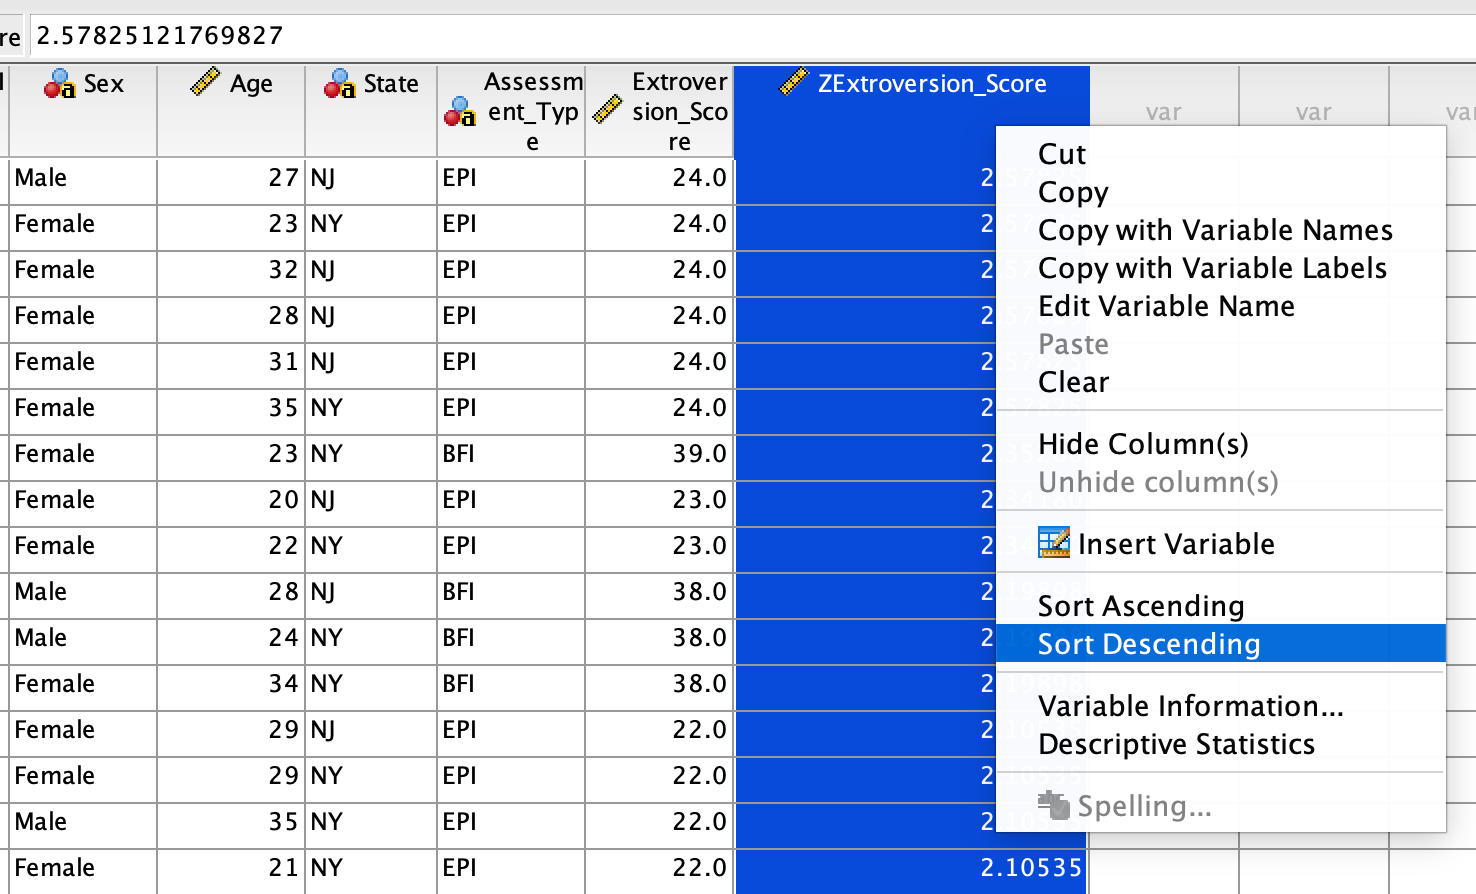
\includegraphics[width=5.75in,height=\textheight,keepaspectratio]{images/lab4_im4.png}
\end{center}

\begin{tcolorbox}[enhanced jigsaw, opacityback=0, coltitle=black, title=\textcolor{quarto-callout-tip-color}{\faLightbulb}\hspace{0.5em}{Checkpoint 2}, titlerule=0mm, rightrule=.15mm, toprule=.15mm, opacitybacktitle=0.6, colbacktitle=quarto-callout-tip-color!10!white, colback=white, bottomtitle=1mm, arc=.35mm, toptitle=1mm, bottomrule=.15mm, colframe=quarto-callout-tip-color-frame, breakable, leftrule=.75mm, left=2mm]

Who are the top ten most extroverted individuals? Record their
\texttt{Applicant\_ID}'s, the assessment they took (BFI or EPI) and
\texttt{ZExtroversion\_Scores}.

\end{tcolorbox}

\subsection{Part 3 --- Characteristics of
Z-scores}\label{part-3-characteristics-of-z-scores}

\subsubsection{Mean and Standard
Deviation}\label{mean-and-standard-deviation}

We want to explore the \textbf{mean} and \textbf{standard deviation} of
the \(z-scores\) for each assessment. To do this, follow the steps
below:

\begin{itemize}
\tightlist
\item
  Go to \textbf{Analyze} \textgreater{} \textbf{Descriptive
  Statistics}\textgreater{}\textbf{Explore}
\item
  Move \texttt{Assessment\_Type} into the \textbf{Factor List} and
  \texttt{ZExtroversion\_Score} into the \textbf{Dependent List}.
\item
  Select \textbf{Statistics}
\end{itemize}

Your set up should look as shown below:

\begin{center}
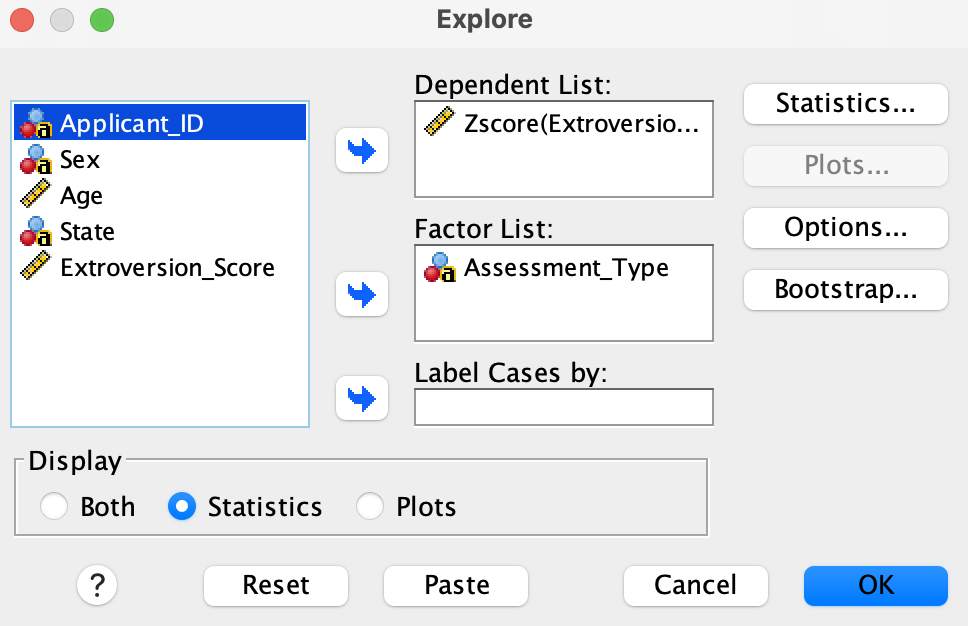
\includegraphics[width=5.75in,height=\textheight,keepaspectratio]{images/lab4_im2.png}
\end{center}

\begin{itemize}
\tightlist
\item
  Click \textbf{OK}.
\end{itemize}

\begin{tcolorbox}[enhanced jigsaw, opacityback=0, coltitle=black, title=\textcolor{quarto-callout-tip-color}{\faLightbulb}\hspace{0.5em}{Checkpoint}, titlerule=0mm, rightrule=.15mm, toprule=.15mm, opacitybacktitle=0.6, colbacktitle=quarto-callout-tip-color!10!white, colback=white, bottomtitle=1mm, arc=.35mm, toptitle=1mm, bottomrule=.15mm, colframe=quarto-callout-tip-color-frame, breakable, leftrule=.75mm, left=2mm]

What do you notice about the mean and standard deviation of the
\(z-scores\)? Would you expect this to be the case every time we convert
any set of scores to Z-scores? Explain.

\end{tcolorbox}

\subsubsection{Examining the Distributions (Shape) of
Z-scores}\label{examining-the-distributions-shape-of-z-scores}

There is a common misconception that z-scores (standardized scores) are
always normally distributed. We will show that this claim is not true by
creating histograms for the original assessments and compare them to the
histograms of the corresponding \(z-scores\).

\begin{itemize}
\item
  Go to \textbf{Graphs} \textgreater{} \textbf{Chart Builder}
  \textgreater{} \textbf{Histogram}.
\item
  Move \texttt{Extroversion\_Score} into the \textbf{Variable} box and
  \texttt{Assessment\_Type} into the \textbf{Panel} box under
  \texttt{Rows}. Your set up should look as shown below:

  \begin{center}
  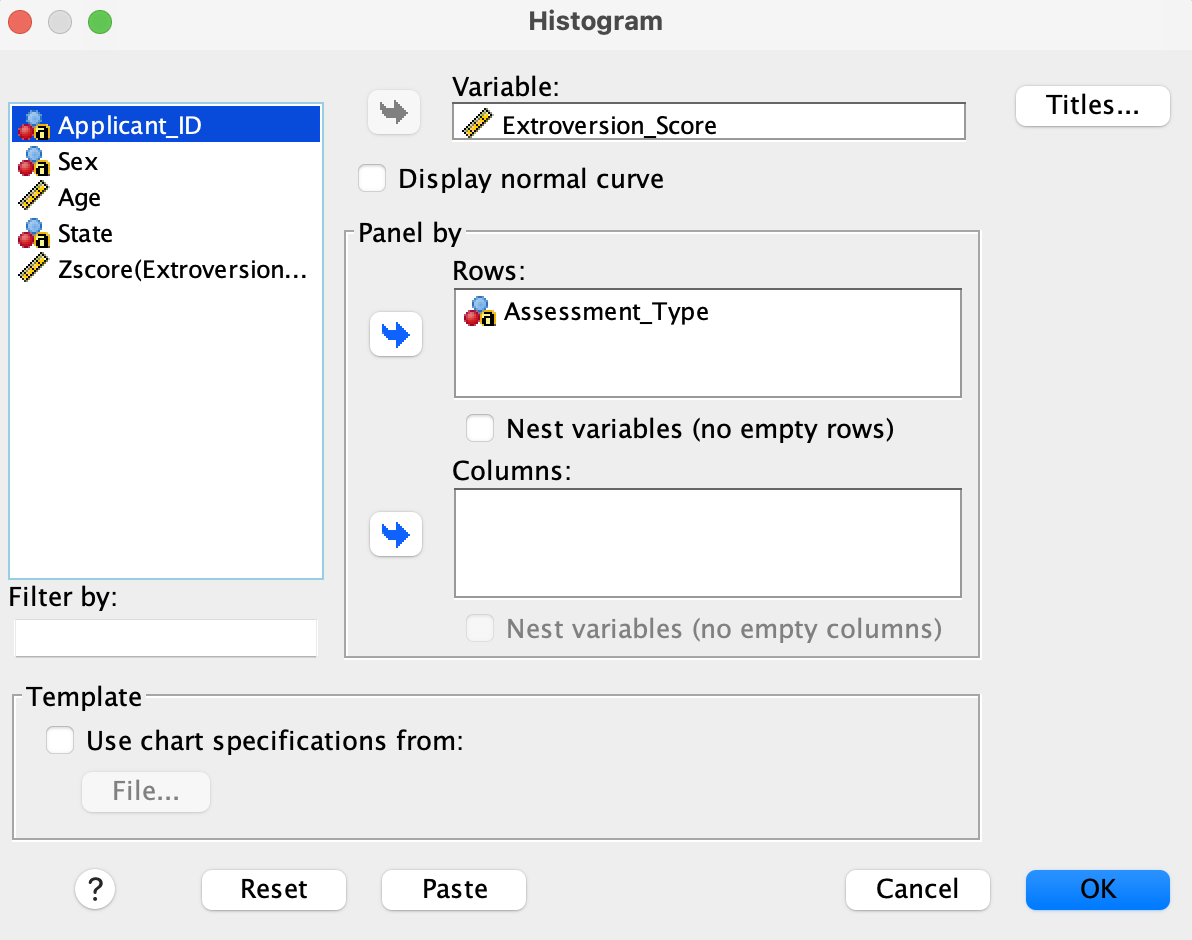
\includegraphics[width=5.61458in,height=\textheight,keepaspectratio]{images/lab4_im3.png}
  \end{center}
\item
  Click \textbf{OK}.
\end{itemize}

Now repeat the above process but this time use
\texttt{ZExtroversion\_Score} instead of \texttt{Extroversion\_Score}.
Your set up should look as shown below:

\begin{tcolorbox}[enhanced jigsaw, opacityback=0, coltitle=black, title=\textcolor{quarto-callout-tip-color}{\faLightbulb}\hspace{0.5em}{``Checkpoint}, titlerule=0mm, rightrule=.15mm, toprule=.15mm, opacitybacktitle=0.6, colbacktitle=quarto-callout-tip-color!10!white, colback=white, bottomtitle=1mm, arc=.35mm, toptitle=1mm, bottomrule=.15mm, colframe=quarto-callout-tip-color-frame, breakable, leftrule=.75mm, left=2mm]

How would you describe the distribution of the original extroversion
scores for each assessment? How do these compare to the distribution of
the \(z-scores\)?

\end{tcolorbox}

\subsection{Part 4 --- The Standard Normal
Distribution}\label{part-4-the-standard-normal-distribution}

The standard normal distribution is a special case of the \textbf{normal
distribution} with a mean of 0 and a standard deviation of 1. It is a
theoretical distribution that researchers commonly use to examine how
well a set of data fits the normal distribution. Below is a screenshot
of the standard normal distribution.

\begin{figure}[H]

{\centering 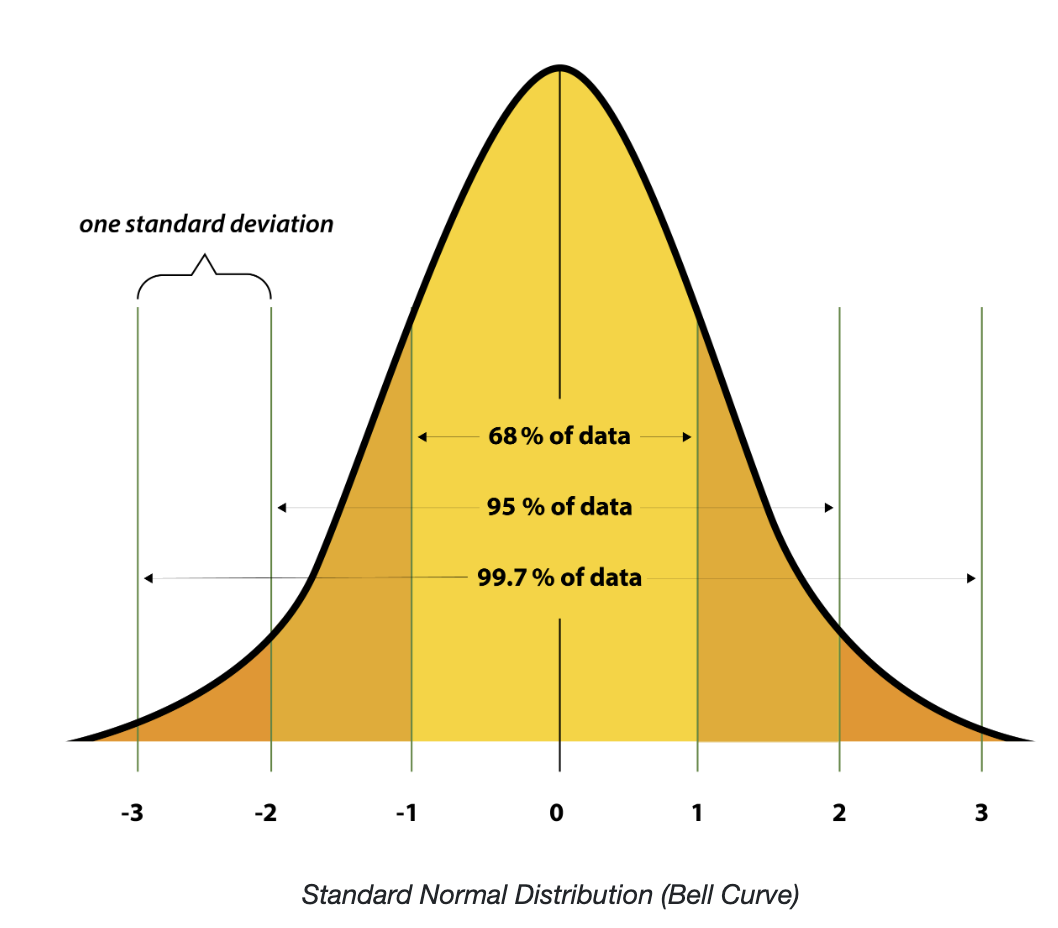
\includegraphics[width=5.40625in,height=\textheight,keepaspectratio]{images/lab4_im1.png}

}

\caption{Source: National Library of Medicine}

\end{figure}%

\begin{tcolorbox}[enhanced jigsaw, opacityback=0, coltitle=black, title=\textcolor{quarto-callout-note-color}{\faInfo}\hspace{0.5em}{Important Notes about the Standard Normal Distribution}, titlerule=0mm, rightrule=.15mm, toprule=.15mm, opacitybacktitle=0.6, colbacktitle=quarto-callout-note-color!10!white, colback=white, bottomtitle=1mm, arc=.35mm, toptitle=1mm, bottomrule=.15mm, colframe=quarto-callout-note-color-frame, breakable, leftrule=.75mm, left=2mm]

\begin{itemize}
\tightlist
\item
  The mean, median, and mode are all equal to 0 (center of the
  distribution).
\item
  The distribution is bell-shaped and symmetric about the mean.
\item
  The standard deviation is equal to 1.
\item
  95\% of the data falls within 2 standard deviations; while 99.7\%
  (nearly all data) falls within 3 standard deviations of the mean.
\item
  The further you go from the mean in either direction, the less likely
  you are to find data points in that region. Data that that are more
  than 2 sd's from the mean are very unlikely while those beyond 3
  standard deviations can be considered outliers.
\end{itemize}

\end{tcolorbox}

\subsection{Take-Home Lab Exercises}\label{take-home-lab-exercises}

Before beginning the lab, you will need to undo the \textbf{split file}
option that was enabled earlier by going to \textbf{Data} \textgreater{}
\textbf{Split File} \textgreater{} \textbf{Analyze all cases, do not
create groups} \textgreater{} \textbf{OK}. Some exercises here may
require use of \textbf{split file}, so you will need to repeat the steps
above to split the file again when necessary.

\begin{enumerate}
\def\labelenumi{\arabic{enumi}.}
\tightlist
\item
  Make a box plot to visualize the \texttt{Age} variable. Based on this
  box plot, a student claims that the ages of the applicants are
  ``normally distributed''. Would you agree with this claim? Why or why
  not?
\item
  Use SPSS to find the top 10 most extroverted females in the data.
  Record their \texttt{Applicant\_ID\textquotesingle{}}s and describe
  the steps you took in SPSS to find them.
\item
  Using SPSS, find the 10 most extroverted individuals from New Jersey.
  Record their \texttt{Applicant\_ID} and describe the steps you took in
  SPSS to solve this problem.
\item
  Suppose we want to find the 10 most extroverted individuals aged
  between 20 and 30 years old (inclusive). Use SPSS to solve this
  problem and briefly describe your steps.
\end{enumerate}

\subsection{Submission Checklist}\label{submission-checklist}

\begin{itemize}
\tightlist
\item[$\square$]
  A saved SPSS data (.sav) file showing the variables and data (includes
  \(z-scores\)).
\item[$\square$]
  SPSS output file (.spv) showing the analyses performed.
\item[$\square$]
  Completed responses for the Questions above. This document should be
  typed (Times New Roman, Font size 12, double spaced). The document
  should include necessary SPSS output tables and graphs. Remember that
  SPSS output tables and graphs can be copied and pasted into a word
  document.
\end{itemize}




\end{document}
